% Created by tikzDevice version 0.10.1 on 2018-06-14 11:49:29
% !TEX encoding = UTF-8 Unicode
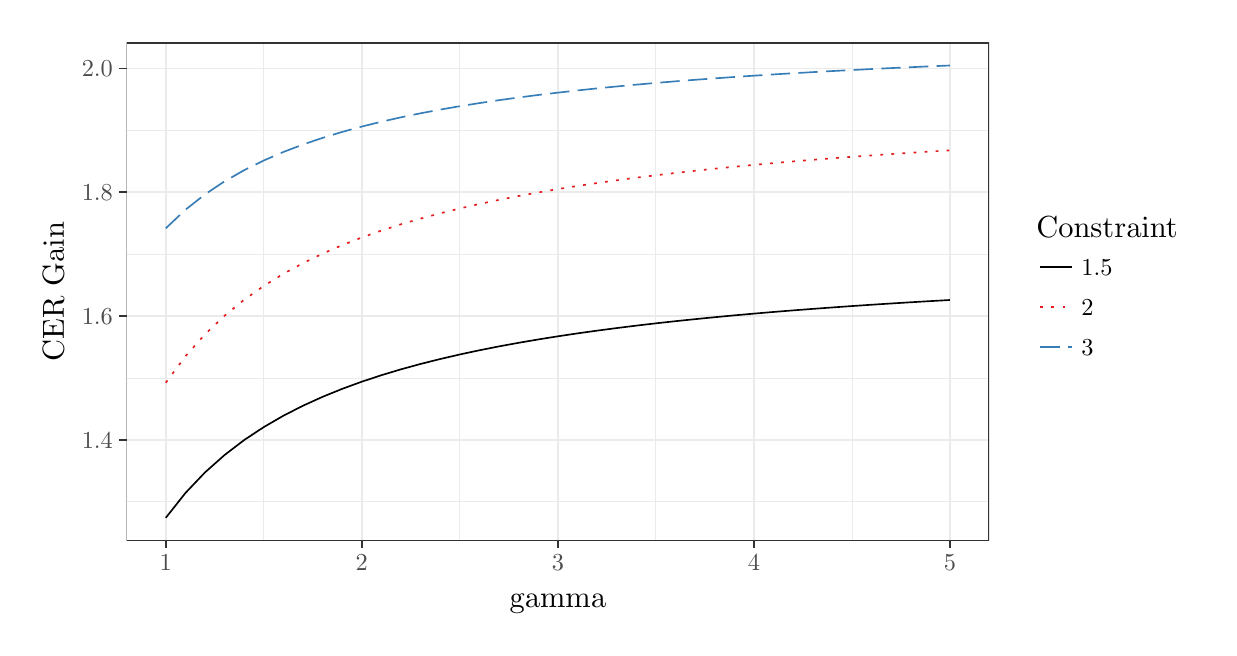
\begin{tikzpicture}[x=1pt,y=1pt]
\definecolor{fillColor}{RGB}{255,255,255}
\path[use as bounding box,fill=fillColor,fill opacity=0.00] (0,0) rectangle (426.79,216.81);
\begin{scope}
\path[clip] (  0.00,  0.00) rectangle (426.79,216.81);
\definecolor{drawColor}{RGB}{255,255,255}
\definecolor{fillColor}{RGB}{255,255,255}

\path[draw=drawColor,line width= 0.6pt,line join=round,line cap=round,fill=fillColor] (  0.00,  0.00) rectangle (426.79,216.81);
\end{scope}
\begin{scope}
\path[clip] ( 35.74, 31.53) rectangle (347.42,211.31);
\definecolor{fillColor}{RGB}{255,255,255}

\path[fill=fillColor] ( 35.74, 31.53) rectangle (347.42,211.31);
\definecolor{drawColor}{gray}{0.92}

\path[draw=drawColor,line width= 0.3pt,line join=round] ( 35.74, 45.51) --
	(347.42, 45.51);

\path[draw=drawColor,line width= 0.3pt,line join=round] ( 35.74, 90.23) --
	(347.42, 90.23);

\path[draw=drawColor,line width= 0.3pt,line join=round] ( 35.74,134.95) --
	(347.42,134.95);

\path[draw=drawColor,line width= 0.3pt,line join=round] ( 35.74,179.67) --
	(347.42,179.67);

\path[draw=drawColor,line width= 0.3pt,line join=round] ( 85.33, 31.53) --
	( 85.33,211.31);

\path[draw=drawColor,line width= 0.3pt,line join=round] (156.16, 31.53) --
	(156.16,211.31);

\path[draw=drawColor,line width= 0.3pt,line join=round] (227.00, 31.53) --
	(227.00,211.31);

\path[draw=drawColor,line width= 0.3pt,line join=round] (297.84, 31.53) --
	(297.84,211.31);

\path[draw=drawColor,line width= 0.6pt,line join=round] ( 35.74, 67.87) --
	(347.42, 67.87);

\path[draw=drawColor,line width= 0.6pt,line join=round] ( 35.74,112.59) --
	(347.42,112.59);

\path[draw=drawColor,line width= 0.6pt,line join=round] ( 35.74,157.31) --
	(347.42,157.31);

\path[draw=drawColor,line width= 0.6pt,line join=round] ( 35.74,202.03) --
	(347.42,202.03);

\path[draw=drawColor,line width= 0.6pt,line join=round] ( 49.91, 31.53) --
	( 49.91,211.31);

\path[draw=drawColor,line width= 0.6pt,line join=round] (120.74, 31.53) --
	(120.74,211.31);

\path[draw=drawColor,line width= 0.6pt,line join=round] (191.58, 31.53) --
	(191.58,211.31);

\path[draw=drawColor,line width= 0.6pt,line join=round] (262.42, 31.53) --
	(262.42,211.31);

\path[draw=drawColor,line width= 0.6pt,line join=round] (333.25, 31.53) --
	(333.25,211.31);
\definecolor{drawColor}{RGB}{0,0,0}

\path[draw=drawColor,line width= 0.6pt,line join=round] ( 49.91, 39.70) --
	( 56.99, 48.65) --
	( 64.07, 56.10) --
	( 71.16, 62.40) --
	( 78.24, 67.81) --
	( 85.33, 72.49) --
	( 92.41, 76.59) --
	( 99.49, 80.21) --
	(106.58, 83.42) --
	(113.66, 86.30) --
	(120.74, 88.89) --
	(127.83, 91.23) --
	(134.91, 93.36) --
	(141.99, 95.30) --
	(149.08, 97.08) --
	(156.16, 98.72) --
	(163.25,100.24) --
	(170.33,101.64) --
	(177.41,102.94) --
	(184.50,104.15) --
	(191.58,105.28) --
	(198.66,106.34) --
	(205.75,107.33) --
	(212.83,108.26) --
	(219.92,109.14) --
	(227.00,109.97) --
	(234.08,110.75) --
	(241.17,111.48) --
	(248.25,112.18) --
	(255.33,112.85) --
	(262.42,113.48) --
	(269.50,114.08) --
	(276.58,114.65) --
	(283.67,115.19) --
	(290.75,115.71) --
	(297.84,116.21) --
	(304.92,116.69) --
	(312.00,117.14) --
	(319.09,117.58) --
	(326.17,118.00) --
	(333.25,118.40);
\definecolor{drawColor}{RGB}{228,26,28}

\path[draw=drawColor,line width= 0.6pt,dash pattern=on 1pt off 3pt ,line join=round] ( 49.91, 88.51) --
	( 56.99, 98.05) --
	( 64.07,106.00) --
	( 71.16,112.73) --
	( 78.24,118.50) --
	( 85.33,123.49) --
	( 92.41,127.87) --
	( 99.49,131.73) --
	(106.58,135.16) --
	(113.66,138.23) --
	(120.74,140.99) --
	(127.83,143.49) --
	(134.91,145.76) --
	(141.99,147.83) --
	(149.08,149.73) --
	(156.16,151.48) --
	(163.25,153.10) --
	(170.33,154.59) --
	(177.41,155.98) --
	(184.50,157.27) --
	(191.58,158.48) --
	(198.66,159.61) --
	(205.75,160.67) --
	(212.83,161.66) --
	(219.92,162.60) --
	(227.00,163.48) --
	(234.08,164.31) --
	(241.17,165.10) --
	(248.25,165.85) --
	(255.33,166.55) --
	(262.42,167.23) --
	(269.50,167.87) --
	(276.58,168.48) --
	(283.67,169.06) --
	(290.75,169.61) --
	(297.84,170.14) --
	(304.92,170.65) --
	(312.00,171.14) --
	(319.09,171.60) --
	(326.17,172.05) --
	(333.25,172.48);
\definecolor{drawColor}{RGB}{55,126,184}

\path[draw=drawColor,line width= 0.6pt,dash pattern=on 7pt off 3pt ,line join=round] ( 49.91,144.31) --
	( 56.99,151.00) --
	( 64.07,156.57) --
	( 71.16,161.28) --
	( 78.24,165.32) --
	( 85.33,168.82) --
	( 92.41,171.89) --
	( 99.49,174.59) --
	(106.58,176.99) --
	(113.66,179.14) --
	(120.74,181.08) --
	(127.83,182.83) --
	(134.91,184.42) --
	(141.99,185.87) --
	(149.08,187.21) --
	(156.16,188.43) --
	(163.25,189.56) --
	(170.33,190.61) --
	(177.41,191.58) --
	(184.50,192.49) --
	(191.58,193.33) --
	(198.66,194.12) --
	(205.75,194.87) --
	(212.83,195.56) --
	(219.92,196.22) --
	(227.00,196.84) --
	(234.08,197.42) --
	(241.17,197.97) --
	(248.25,198.49) --
	(255.33,198.99) --
	(262.42,199.46) --
	(269.50,199.91) --
	(276.58,200.34) --
	(283.67,200.74) --
	(290.75,201.13) --
	(297.84,201.50) --
	(304.92,201.86) --
	(312.00,202.20) --
	(319.09,202.53) --
	(326.17,202.84) --
	(333.25,203.14);
\definecolor{drawColor}{gray}{0.20}

\path[draw=drawColor,line width= 0.6pt,line join=round,line cap=round] ( 35.74, 31.53) rectangle (347.42,211.31);
\end{scope}
\begin{scope}
\path[clip] (  0.00,  0.00) rectangle (426.79,216.81);
\definecolor{drawColor}{gray}{0.30}

\node[text=drawColor,anchor=base east,inner sep=0pt, outer sep=0pt, scale=  0.88] at ( 30.79, 64.84) {1.4};

\node[text=drawColor,anchor=base east,inner sep=0pt, outer sep=0pt, scale=  0.88] at ( 30.79,109.56) {1.6};

\node[text=drawColor,anchor=base east,inner sep=0pt, outer sep=0pt, scale=  0.88] at ( 30.79,154.28) {1.8};

\node[text=drawColor,anchor=base east,inner sep=0pt, outer sep=0pt, scale=  0.88] at ( 30.79,199.00) {2.0};
\end{scope}
\begin{scope}
\path[clip] (  0.00,  0.00) rectangle (426.79,216.81);
\definecolor{drawColor}{gray}{0.20}

\path[draw=drawColor,line width= 0.6pt,line join=round] ( 32.99, 67.87) --
	( 35.74, 67.87);

\path[draw=drawColor,line width= 0.6pt,line join=round] ( 32.99,112.59) --
	( 35.74,112.59);

\path[draw=drawColor,line width= 0.6pt,line join=round] ( 32.99,157.31) --
	( 35.74,157.31);

\path[draw=drawColor,line width= 0.6pt,line join=round] ( 32.99,202.03) --
	( 35.74,202.03);
\end{scope}
\begin{scope}
\path[clip] (  0.00,  0.00) rectangle (426.79,216.81);
\definecolor{drawColor}{gray}{0.20}

\path[draw=drawColor,line width= 0.6pt,line join=round] ( 49.91, 28.78) --
	( 49.91, 31.53);

\path[draw=drawColor,line width= 0.6pt,line join=round] (120.74, 28.78) --
	(120.74, 31.53);

\path[draw=drawColor,line width= 0.6pt,line join=round] (191.58, 28.78) --
	(191.58, 31.53);

\path[draw=drawColor,line width= 0.6pt,line join=round] (262.42, 28.78) --
	(262.42, 31.53);

\path[draw=drawColor,line width= 0.6pt,line join=round] (333.25, 28.78) --
	(333.25, 31.53);
\end{scope}
\begin{scope}
\path[clip] (  0.00,  0.00) rectangle (426.79,216.81);
\definecolor{drawColor}{gray}{0.30}

\node[text=drawColor,anchor=base,inner sep=0pt, outer sep=0pt, scale=  0.88] at ( 49.91, 20.52) {1};

\node[text=drawColor,anchor=base,inner sep=0pt, outer sep=0pt, scale=  0.88] at (120.74, 20.52) {2};

\node[text=drawColor,anchor=base,inner sep=0pt, outer sep=0pt, scale=  0.88] at (191.58, 20.52) {3};

\node[text=drawColor,anchor=base,inner sep=0pt, outer sep=0pt, scale=  0.88] at (262.42, 20.52) {4};

\node[text=drawColor,anchor=base,inner sep=0pt, outer sep=0pt, scale=  0.88] at (333.25, 20.52) {5};
\end{scope}
\begin{scope}
\path[clip] (  0.00,  0.00) rectangle (426.79,216.81);
\definecolor{drawColor}{RGB}{0,0,0}

\node[text=drawColor,anchor=base,inner sep=0pt, outer sep=0pt, scale=  1.10] at (191.58,  7.44) {gamma};
\end{scope}
\begin{scope}
\path[clip] (  0.00,  0.00) rectangle (426.79,216.81);
\definecolor{drawColor}{RGB}{0,0,0}

\node[text=drawColor,rotate= 90.00,anchor=base,inner sep=0pt, outer sep=0pt, scale=  1.10] at ( 13.08,121.42) {CER Gain};
\end{scope}
\begin{scope}
\path[clip] (  0.00,  0.00) rectangle (426.79,216.81);
\definecolor{fillColor}{RGB}{255,255,255}

\path[fill=fillColor] (358.80, 88.45) rectangle (421.29,154.39);
\end{scope}
\begin{scope}
\path[clip] (  0.00,  0.00) rectangle (426.79,216.81);
\definecolor{drawColor}{RGB}{0,0,0}

\node[text=drawColor,anchor=base west,inner sep=0pt, outer sep=0pt, scale=  1.10] at (364.49,141.12) {Constraint};
\end{scope}
\begin{scope}
\path[clip] (  0.00,  0.00) rectangle (426.79,216.81);
\definecolor{fillColor}{RGB}{255,255,255}

\path[fill=fillColor] (364.49,123.05) rectangle (378.95,137.51);
\end{scope}
\begin{scope}
\path[clip] (  0.00,  0.00) rectangle (426.79,216.81);
\definecolor{drawColor}{RGB}{0,0,0}

\path[draw=drawColor,line width= 0.6pt,line join=round] (365.94,130.28) -- (377.50,130.28);
\end{scope}
\begin{scope}
\path[clip] (  0.00,  0.00) rectangle (426.79,216.81);
\definecolor{fillColor}{RGB}{255,255,255}

\path[fill=fillColor] (364.49,108.60) rectangle (378.95,123.05);
\end{scope}
\begin{scope}
\path[clip] (  0.00,  0.00) rectangle (426.79,216.81);
\definecolor{drawColor}{RGB}{228,26,28}

\path[draw=drawColor,line width= 0.6pt,dash pattern=on 1pt off 3pt ,line join=round] (365.94,115.83) -- (377.50,115.83);
\end{scope}
\begin{scope}
\path[clip] (  0.00,  0.00) rectangle (426.79,216.81);
\definecolor{fillColor}{RGB}{255,255,255}

\path[fill=fillColor] (364.49, 94.14) rectangle (378.95,108.60);
\end{scope}
\begin{scope}
\path[clip] (  0.00,  0.00) rectangle (426.79,216.81);
\definecolor{drawColor}{RGB}{55,126,184}

\path[draw=drawColor,line width= 0.6pt,dash pattern=on 7pt off 3pt ,line join=round] (365.94,101.37) -- (377.50,101.37);
\end{scope}
\begin{scope}
\path[clip] (  0.00,  0.00) rectangle (426.79,216.81);
\definecolor{drawColor}{RGB}{0,0,0}

\node[text=drawColor,anchor=base west,inner sep=0pt, outer sep=0pt, scale=  0.88] at (380.75,127.25) {1.5};
\end{scope}
\begin{scope}
\path[clip] (  0.00,  0.00) rectangle (426.79,216.81);
\definecolor{drawColor}{RGB}{0,0,0}

\node[text=drawColor,anchor=base west,inner sep=0pt, outer sep=0pt, scale=  0.88] at (380.75,112.80) {2};
\end{scope}
\begin{scope}
\path[clip] (  0.00,  0.00) rectangle (426.79,216.81);
\definecolor{drawColor}{RGB}{0,0,0}

\node[text=drawColor,anchor=base west,inner sep=0pt, outer sep=0pt, scale=  0.88] at (380.75, 98.34) {3};
\end{scope}
\end{tikzpicture}
